%Input preamble
%Style
\documentclass[12pt]{article}
\usepackage[top=1in, bottom=1in, left=1in, right=1in]{geometry}
\parindent 22pt
\usepackage{fancyhdr}

%Packages
\usepackage{adjustbox}
\usepackage{amsmath}
\usepackage{amsfonts}
\usepackage{amssymb}
\usepackage{bm}
\usepackage[table]{xcolor}
\usepackage{tabu}
\usepackage{color,soul}
\usepackage{makecell}
\usepackage{longtable}
\usepackage{multirow}
\usepackage[normalem]{ulem}
\usepackage{etoolbox}
\usepackage{graphicx}
\usepackage{tabularx}
\usepackage{ragged2e}
\usepackage{booktabs}
\usepackage{caption}
\usepackage{fixltx2e}
\usepackage[para, flushleft]{threeparttablex}
\usepackage[capposition=top,objectset=centering]{floatrow}
\usepackage{subcaption}
\usepackage{pdfpages}
\usepackage{pdflscape}
\usepackage{natbib}
\usepackage{bibunits}
\definecolor{maroon}{HTML}{990012}
\usepackage[colorlinks=true,linkcolor=maroon,citecolor=maroon,urlcolor=maroon,anchorcolor=maroon]{hyperref}
\usepackage{marvosym}
\usepackage{makeidx}
\usepackage{tikz}
\usetikzlibrary{shapes}
\usepackage{setspace}
\usepackage{enumerate}
\usepackage{rotating}
\usepackage{tocloft}
\usepackage{epstopdf}
\usepackage[titletoc]{appendix}
\usepackage{framed}
\usepackage{comment}
\usepackage{xr}
\usepackage{titlesec}
\usepackage{footnote}
\usepackage{longtable}
\newlength{\tablewidth}
\setlength{\tablewidth}{9.3in}
\setcounter{secnumdepth}{4}

\titleformat{\paragraph}
{\normalfont\normalsize\bfseries}{\theparagraph}{1em}{}
\titlespacing*{\paragraph}
{0pt}{3.25ex plus 1ex minus .2ex}{1.5ex plus .2ex}
\makeatletter
\pretocmd\start@align
{%
  \let\everycr\CT@everycr
  \CT@start
}{}{}
\apptocmd{\endalign}{\CT@end}{}{}
\makeatother
%Watermark
\usepackage[printwatermark]{xwatermark}
\usepackage{lipsum}
\definecolor{lightgray}{RGB}{220,220,220}
%\newwatermark[allpages,color=lightgray,angle=45,scale=3,xpos=0,ypos=0]{Preliminary Draft}

%Further subsection level
\usepackage{titlesec}
\setcounter{secnumdepth}{4}
\titleformat{\paragraph}
{\normalfont\normalsize\bfseries}{\theparagraph}{1em}{}
\titlespacing*{\paragraph}
{0pt}{3.25ex plus 1ex minus .2ex}{1.5ex plus .2ex}

\setcounter{secnumdepth}{5}
\titleformat{\subparagraph}
{\normalfont\normalsize\bfseries}{\thesubparagraph}{1em}{}
\titlespacing*{\subparagraph}
{0pt}{3.25ex plus 1ex minus .2ex}{1.5ex plus .2ex}

%Functions
\DeclareMathOperator{\cov}{Cov}
\DeclareMathOperator{\corr}{Corr}
\DeclareMathOperator{\var}{Var}
\DeclareMathOperator{\plim}{plim}
\DeclareMathOperator*{\argmin}{arg\,min}
\DeclareMathOperator*{\argmax}{arg\,max}

%Math Environments
\newtheorem{theorem}{Theorem}
\newtheorem{claim}{Claim}
\newtheorem{condition}{Condition}
\renewcommand\thecondition{C--\arabic{condition}}
\newtheorem{algorithm}{Algorithm}
\newtheorem{assumption}{Assumption}
\renewcommand\theassumption{A--\arabic{assumption}}
\newtheorem{remark}{Remark}
\renewcommand\theremark{R--\arabic{remark}}
\newtheorem{definition}[theorem]{Definition}
\newtheorem{hypothesis}[theorem]{Hypothesis}
\newtheorem{property}[theorem]{Property}
\newtheorem{example}[theorem]{Example}
\newtheorem{result}[theorem]{Result}
\newenvironment{proof}{\textbf{Proof:}}{$\bullet$}

%Commands
\newcommand\independent{\protect\mathpalette{\protect\independenT}{\perp}}
\def\independenT#1#2{\mathrel{\rlap{$#1#2$}\mkern2mu{#1#2}}}
\newcommand{\overbar}[1]{\mkern 1.5mu\overline{\mkern-1.5mu#1\mkern-1.5mu}\mkern 1.5mu}
\newcommand{\equald}{\ensuremath{\overset{d}{=}}}
\captionsetup[table]{skip=10pt}
%\makeindex

\setlength\parindent{20pt}
\setlength{\parskip}{0pt}

\newcolumntype{L}[1]{>{\raggedright\let\newline\\\arraybackslash\hspace{0pt}}m{#1}}
\newcolumntype{C}[1]{>{\centering\let\newline\\\arraybackslash\hspace{0pt}}m{#1}}
\newcolumntype{R}[1]{>{\raggedleft\let\newline\\\arraybackslash\hspace{0pt}}m{#1}}



%Logo
%\AddToShipoutPictureBG{%
%  \AtPageUpperLeft{\raisebox{-\height}{
\includegraphics[width=1.5cm]{uchicago.png}}}
%}

\newcolumntype{L}[1]{>{\raggedright\let\newline\\\arraybackslash\hspace{0pt}}m{#1}}
\newcolumntype{C}[1]{>{\centering\let\newline\\\arraybackslash\hspace{0pt}}m{#1}}
\newcolumntype{R}[1]{>{\raggedleft\let\newline\\\arraybackslash\hspace{0pt}}m{#1}}

\newcommand{\mr}{\multirow}
\newcommand{\mc}{\multicolumn}

%\newcommand{\comment}[1]{}

%Other parameters
\newcommand{\noutcomes}{95}
\newcommand{\noutcomesexpp}{357}
\newcommand{\noutcomesexpm}{343}
\newcommand{\noutcomesexpf}{355}
\newcommand{\treatsubsabc}{$75\%$}
\newcommand{\treatsubscarec}{$74\%$}
\newcommand{\treatsubscaref}{$63\%$}

%Counts
%Males
\newcommand{\positivem}{$78\%$}
\newcommand{\positivesm}{$29\%$}

%Females
\newcommand{\positivef}{$78\%$}
\newcommand{\positivesf}{$31\%$}

%Counts, control substitution
%Males
\newcommand{\positivecsnm}{$47\%$}
\newcommand{\positivescsnm}{$15\%$}

\newcommand{\positivecsam}{$79\%$}
\newcommand{\positivescsam}{$29\%$}

%Females
%% no alternative
\newcommand{\positivecsnf}{$84\%$}
\newcommand{\positivescsnf}{$55\%$}

%% alternative
\newcommand{\positivecsaf}{$79\%$}
\newcommand{\positivescsaf}{$33\%$}

%Pooled

%Effects
%Males

%Females
\newcommand{\empf}{$8$}
\newcommand{\yearsedf}{$1.7$}



%Pooled

%CBA
%IRR
%Males
\newcommand{\irrm}{$15\%$}
\newcommand{\irrsem}{$5\%$}

%Females
\newcommand{\irrf}{$9\%$}
\newcommand{\irrsef}{$7\%$}

%Pooled
\newcommand{\irrp}{$13\%$}
\newcommand{\irrsep}{$5\%$}

%BC
%Males
\newcommand{\bcm}{$11.24$}
\newcommand{\bcsem}{$4.60$}

%Females
\newcommand{\bcf}{$2.35$}
\newcommand{\bcsef}{$1.09$}

%Pooled
\newcommand{\bcp}{$5.63$}
\newcommand{\bcsep}{$2.15$}

%NPV streams
%Pooled
\newcommand{\parincomenpvp}{$\$119,346$}

\externaldocument{abc_comprehensivecba_appendix_2016-07-31a_jlg}
\pagenumbering{roman}

\begin{document}

\begin{titlepage}

\title{\Large \textbf{The Long-Term Economic and Social Benefits of an Influential Early Childhood Intervention\\ HOLDING TANK}}

\author{
Jorge Luis Garc\'{i}a\\
The University of Chicago \and
James J. Heckman \\
American Bar Foundation \\
The University of Chicago \and
Andr\'{e}s Hojman\\
The University of Chicago \and
Duncan Ermini Leaf \\
University of Southern California \and
Mar\'{i}a Jos\'{e} Prados \\
University of Southern California \and
Joshua Shea \\
The University of Chicago \and
Jake C. Torcasso\\
The University of Chicago}
\date{First Draft: January 5, 2016\\ This Draft: \today}

\maketitle

\end{titlepage}

\clearpage

\doublespacing

\setcounter{page}{0}
\pagenumbering{arabic}\

\noindent Outline of the paper

\begin{enumerate}[(1)]
\item Intense and growing interest in early childhood programs to promote social mobility and economic/social advantage
\item ABC/CARE
    \begin{enumerate}[(a)]
    \item Targets disadvantaged kids
    \item Starts early (8 weeks)/intensive
    \item Prototype for many successor programs currently in place around the world
        \begin{enumerate}[(i)]
        \item IHDP
        \item Early Head Start
        \item Sparling's list (Australia)
        \end{enumerate}
    \item Many children eligible for it in U.S. (19\% of all African-American children)
    \item Documented to have health benefits (not previously accounted and other benefits (Campbell))
    \item Childcare costs:
        \begin{enumerate}[(i)]
        \item Wage growth of women (sustain according to Gladden and Taber)
        \item Leisure foregone
        \item Educational attainment
        \item Costs of inadequate childcare (what is next best)
        \end{enumerate}
    \end{enumerate}
\item Multiple benefits of the program --- goal is to chronicle benefits and place them in a common metric
    \begin{enumerate}[(a)]
    \item Organize by category
    \item Look at benefits
    \item Aggregate benefits
    \end{enumerate}
\item Costs
    \begin{enumerate}[(a)]
    \item Fresh examination of costs: new primary sources
    \item Tax costs (if publicly funded) --- deadweight burden
    \end{enumerate}
\item Evaluation through age 34
    \begin{enumerate}[(a)]
    \item Account for substitution bias
    \item Vectors of outcomes
    \item Deal with multiple outcomes
        \begin{enumerate}[(i)]
        \item Step-down
        \item Counts
        \item CBA
        \end{enumerate}
    \end{enumerate}
\item CBA requires projecting future benefits and costs
    \begin{enumerate}[(a)]
    \item Previous approaches: \emph{ad hoc} (use a test score gain and impute earnings) Chetty et al./Kline and Walters
    \item We merge data from multiple sources on earnings, health costs, crime, childcare savings, quality of life
    \item Account for sampling uncertainty
    \item Sensitivity analysis for cases where there is some uncertainty but not quantifiable
    \end{enumerate}
\item Main findings: differ by gender
    \begin{enumerate}[(a)]
    \item Substantial monetary benefits for health and QALY (primarily for men)
    \item Childcare and earnings benefits (link childcare to child benefits)
    \item Crime (for men)
    \item Earnings gains (both)
    \item Education (primarily women)
    \item Effects on IQ
    \end{enumerate}
\end{enumerate}

\noindent Additional Points to Make
\begin{enumerate}[(A)]
\item Criticisms that samples are ``too small'' are incorrect; valid asymptotic inference for this and other papers \textbf{[JJH: Jorge, where do we show this?] [JLG: This is thoroughly documented in the Science paper. Either we make reference to it or we can reproduce the analysis for all the outcomes we consider using permutation- and bootstrapped-based difference. We spent a lot of time making sure the treatment effects and -values we get and Science gets are consistent so this shouldn't be a worry. Let me know if you want to document this or not. It seems that we would be documenting something thoroughly documented elsewhere.]}
\item Gender differences interpretable
\item IQ growth long last; sustained for girls (most of it is done by age 3). \textbf{[JJH: Jorge, is this true?] [JLG: See plots in the 16 and 18 in HO. There are gender differences.][JLG: recall discussion follow-up]}
\item No discussion of school age costs (e.g., special education). \textbf{[JLG: see Section 3, in which this is explicitly documented.]}
\end{enumerate}

There is a growing interest in early childhood education as a means for promoting social mobility.\footnote{\citet{Bajaj_Labaton_2009_ObamaRiskAssets,White_House_2014_Econ_of_EC_Investments,White_House_2014_Fact_Sheet_Press}.} However, comprehensive and methodologically rigorous evidence on its economic benefits is still scarce. Many recent studies: (i) focus on a limited set of outcomes like IQ or achievement test scores that fail to capture the full array of program effects;\footnote{An extreme example is the evaluation of preschool programs using an age-eligibility cutoff. A battery of studies compare children who were just eligible and just ineligible for preschool. They therefore only assess the gains of an additional, earlier year of preschool. This does not represent a comprehensive evaluation approach; it evaluates a specific set of children for a very narrow set of tests and within a time horizon of a single year of treatment. Examples of these studies include: \citet{Gormley_Gayer_2005_JHR,Gormley_Gayer_etal_2005_DP,Weiland_2013_CD_Impacts-of-Pre-K}.} (ii) are based on data from follow-ups that are short-term in nature; (iii) do not correct for program attrition or for non-compliance with assignment treatment;\footnote{Consider the evaluation of Head Start through its randomized controlled trial, the Head Start Impact Study \citep{Puma_Bell_etal_2010_HeadStartImpact}. Comparing subjects in the treatment and the control groups usually yields relatively low gains. This attenuation happens because a substantial proportion of subjects randomized out of the program were enrolled into preschool alternatives, some of being other Head Start centers. Thus, a raw comparison between the treatment- and the control-group subjects does not inform on either the efficiency or the effectiveness of Head Start \emph{per se}. Studies providing a methodology to account for substitution find that Head Start has substantial effects, although they focus on a single, short-term outcome \citep{Kline-Walters_2015_NBER-Evaluating,Feller_Grindal_etal_2016_ComparedtoWhat}.} or (iv) are based on randomized controlled trials with flawed designs.\footnote{An evaluation of the Tennessee Voluntary Prekindergarten is an example \citep{Lipsey_et_al_2013_Tennessee_Kindergrtn_PRI,Lipsey_et_al_2015_Randomized_Control_Trial_PRI}. The researchers designed a randomized controlled trial to evaluate the program. Unfortunately, they asked permission to assess the children after the randomization protocol. Thus, their main evaluation is based on information for children whose parents agreed for them to be evaluated \textit{post} randomization, inducing a potential imbalance between the children randomized into and out of the program. The evaluation does not account for that. Further, results for this evaluation represent a narrow set of short-term outcomes.}

Current justification for the long-term effectiveness and the efficiency of early childhood education in the U.S. is largely based on evidence from the Perry Preschool Program (hereafter Perry). This program has a followup to age 40. Analyses of Perry suggest that early childhood education has significant positive effects on a variety of outcomes, even when accounting for compromised randomization, small-sample-size inference, and multiple hypothesis testing.\footnote{\cite{Heckman_Moon_etal_2010_QE}.} The rate of return through age 4- ranges from 7 to 10 percent.\footnote{That is, if one dollar were to be invested at age 4, and then reinvested annually and compounded over a lifetime, the return would accrue to 60 to 300 dollars by age 65. This accounts for both the program's cost and the social burden a government would cause by raising taxes to pay for it \citep{Heckman_Moon_etal_2010_RateofReturn}.} This paper contributes to the literature by analyzing data from two randomized controlled trials, the Carolina Abecedarian Project (ABC) and the Carolina Approach to Responsive Education (CARE). We supplement data using multiple non-experimental, nationally representative sources.

ABC and CARE were programs implemented in the 1970s and early 1980s. Participants are followed through age 34 The programs were separated into two phases. In the first phase of both programs, participants were randomly assigned to high-quality center-based childcare from ages 8 weeks old to 5. The subjects in CARE assigned to center-based childcare in CARE also received home visits that aimed to foster the relationship between the subjects and their parents. Furthermore, CARE incorporated a second treatment group that received home visits without center-based childcare from ages 0 to 5. The second phase of treatment, from ages 5 to 8, consisted of home visits that aimed to continue promoting childhood development. In ABC, the second-phase treatment was randomly assigned independently of the first-phase randomization. In CARE, the second-phase was not randomized; subjects initially randomized to either of the treatment groups maintained their assignment.\footnote{Our main evidence is based on the first-phase component that the two programs share: high-quality center-based childcare.}

The experimental data from ABC and CARE include measures of cognitive and socio-emotional skills, educational and labor market outcomes, administrative criminal records, and a full medical examination when subjects reached their mid-30s. Data from administrative criminal records and from the full medical panel are novel to the literature evaluating early childhood education programs. The non-experimental, nationally representative data include sources to forecast life-cycle gains in public-transfer and labor income, health, and crime. Examples of these sources include: the Medical Expenditure Panel Survey (MEPS), the Medicare Current Beneficiary Survey (MCBS), and the Uniform Crime Reporting Statistics (UCRS).

Our ultimate goal is to provide a cost-benefit analysis of early childhood education programs. To construct this, we proceed in three steps. In the first step, we begin by defining the treatment-effect parameters while we estimate and state how they link to different policy questions. Our methodology accounts for different forms of attrition and non-compliance. Specifically, it considers that the parents of roughly 70\% of the children randomized out of center-based childcare enrolled their children in relatively high-quality preschool alternatives. We refer to this phenomenon as control substitution.\footnote{Control  substitution was not an issue in Perry. Informal conversations with Perry's staff indicate that there were no alternative preschools in the area in which subjects were treated during that time---Ypsilanti, Michigan during the 1960s. This issue is more pressing when evaluating recent programs. Examples include both ABC and Head Start---see \citep{Puma_Bell_etal_2010_HeadStartImpact} for a documentation of treatment substitution in the Head Start Impact Study.}\\

In the second and intermediate step, we provide treatment-effect estimates for a wide variety of outcomes. In doing so, a challenge arises: multiple hypothesis testing. We account for this in a standard way \citep{Lehman_Romano_2005_AnnStat,Romano_Shaikh_2006_AnnStat} while noting that it is often the case that arbitrary blocks need to be formed in order to adjust the inference using the step-down procedure. We propose and formalize an alternative: count the positive (and significant) treatment effects across the outcomes we consider. This crude summary highlights which outcome categories have the most effects, and therefore are relevant to the cost-benefit analysis, which then weighs the relative importance of each outcome.

Finally, to conduct the cost-benefit analysis, we combine the experimental and non-experimental sources of data to forecast and monetize parental income, transfer income, labor income, education, health, and crime outcomes over the life-cycle to provide estimates of the benefit-to-cost ratio and the internal rate of return of early childhood education. Because these statistics summarize the effectiveness of a program accounting for all its components in a single statistic (and a single inference test), they provide a comprehensive solution for the challenge of performing multiple hypothesis testing.

ABC's and CARE's center-based childcare from ages 0 to 5 as implemented, had substantial treatment effects on a comprehensive set of measures of human development from childhood through adulthood. For females, \positivef\ of the outcomes we study have a \textit{positive} average treatment effect; \positivesf\ of the outcomes we study have a \textit{positive and significant} average treatment effect, at the 10\% level. For males, the analogous figures are \positivem\ and \positivesm.\footnote{These results account for program attrition.} The effects strengthen when accounting for control substitution by the families of the subjects who were randomized out of the main treatment  the programs offered.

This paper extends the work of \citet{Campbell_Conti_etal_2014_EarlyChildhoodInvestments}, who analyze the effectiveness of ABC at improving long-term health outcomes. We extend the analysis by (i) assessing multiple measures of human development; (ii) accounting for control substitution; and (iii) providing an alternative to test multiple hypotheses.\footnote{\cite{Campbell_Pungello_etal_2012_DP} also precede our work. The authors estimate treatment effects on adulthood outcomes in ABC. Unlike our approach, the authors do not assess outcomes such as health status, criminal behavior, and socio-emotional skills.} Furthermore, we complement the analysis by studying ABC together with CARE.

The cost-benefit analysis of ABC and CARE provide composite measures of the program's efficiency that weigh these treatment effects according to their cost to society. The pooled benefit-to-cost ratio, \bcp\ (s.e. \bcsep), and internal rate of return \irrp\ (s.e. \irrsep), indicate that ABC and CARE are an efficient program when considering the life-cycle trajectories of the subjects.

Two previous related pieces of work provide a cost-benefit analysis of ABC \citep{Masse_Barnett_2002_BOOKBenefitCostAnalysis,Barnett_Masse_2007_EER}. Their analysis is limited to outcomes up to age 21, before any of the labor income, crime, and health benefits of the program arise according to our findings. It does not provide standard errors or an analysis of the estimates' sensitivity to different modeling assumptions. \citet{Kline-Walters_2015_NBER-Evaluating} provide a back-of-the-envelope cost-benefit analysis of Head Start using the Head Start Impact Study. They do not analyze the life-cycle benefits and costs of early childhood education.

The paper proceeds as follows. Section~\ref{section:background}  provides an overview of each program. It includes a description of the eligibility criteria and the populations served, a characterization of the randomization protocol and control substitution, a comprehensive summary of the treatment, and a description of the data sources. Section~\ref{section:methodology} formalizes our methodology by discussing how we correct for compromised randomization and control substitution, how we test for treatment effects across multiple outcomes, and how we forecast outcomes across the life cycle. Section~\ref{section:results} presents our main results. Section~\ref{section:conclusion} concludes. An extensive appendix presents a thorough description of the program and its costs, the data, and details on how we monetize the life-cycle outcomes. It also discusses various alternative methodologies to evaluate the programs, and documents the results we present to a further extent.

\begin{figure}[H]
		\caption{Control Substitution, ABC} \label{fig:treatsubabc}
		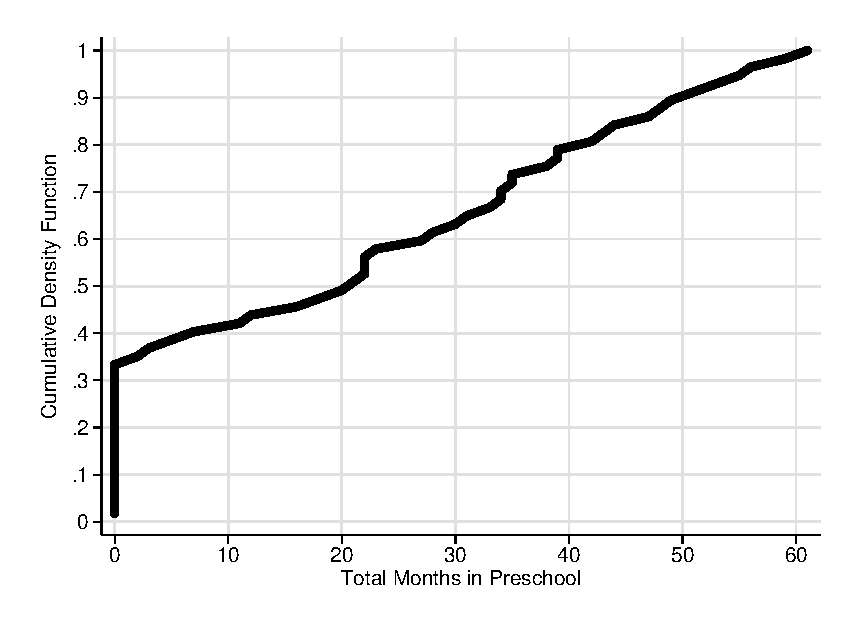
\includegraphics[width=.9\columnwidth]{output/abc_controlcontamination_months.eps}
\floatfoot{
\footnotesize
\noindent Note: This figure displays the cumulative density function of enrollment in alternative preschools of the control group in ABC.}
\end{figure}


%References
\singlespace
\bibliographystyle{chicago}
\bibliography{heckman}

\end{document} 